Data extracted is a method to gather data for analysing and predicting tasks. Data-driven is a method based on which features can be extracted from the historical data to~\cite{SMARRA20181252}. In classification and prediction problems, it is essential to discover the pattern of the data to get insights. Ensemble learning algorithms and Neural Networks are been found effective~\cite{10.1145/3414274.3414278, RB2021} for real-world pattern detection. This is, however, extremely hard to identify the target information from institutions data and identify patterns to classify the problem. 

The purpose of the chapter is to extract information from a historical dataset and find a suitable classifier for anomaly detection. 



To implement The data-driven machine learning technique that detects suspicious companies to prevent trade-credit fraud, the below system design was used. The design is broadly broken down into main three components. These are Data Mining, Model Configuration, and Model selection. In the below sections each of the components is described. 

\begin{figure}[htp]
    \begin{center} 
    \usetikzlibrary{decorations.text} 
    \newcommand*{\mytextstyle}{\sffamily\Large\bfseries\color{black!85}} 
    \newcommand{\arcarrow}[8]{% 
    % inner radius, middle radius, outer radius, start angle, 
    % end angle, tip protusion angle, options, text 
      \pgfmathsetmacro{\rin}{#1} 
      \pgfmathsetmacro{\rmid}{#2} 
      \pgfmathsetmacro{\rout}{#3} 
      \pgfmathsetmacro{\astart}{#4} 
      \pgfmathsetmacro{\aend}{#5} 
      \pgfmathsetmacro{\atip}{#6} 
      \fill[#7] (\astart+\atip:\rin) arc (\astart+\atip:\aend:\rin) 
           -- (\aend-\atip:\rmid) 
           -- (\aend:\rout) arc (\aend:\astart+\atip:\rout) 
           -- (\astart:\rmid) -- cycle; 
      \path[font = \sffamily, decoration = {text along path, text = {|\mytextstyle|#8}, 
        text align = {align = center}, raise = -.8ex}, decorate] 
        (\astart+\atip:\rmid) arc (\astart+\atip:\aend+\atip:\rmid); 
    } 
    
    \definecolor{grau}{RGB}{208,208,208} 
    \definecolor{mymagenta}{RGB}{226,0,116} 

        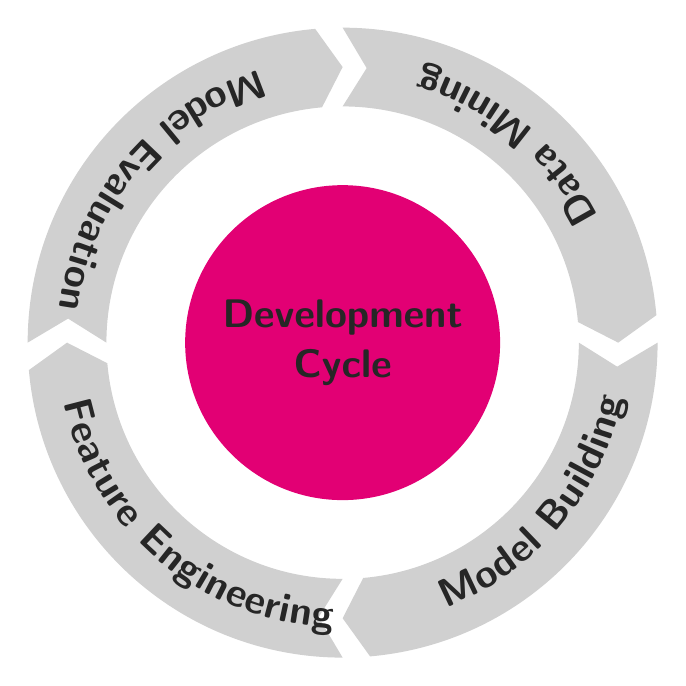
\begin{tikzpicture} 
        \fill[even odd rule,mymagenta] circle (2.0); 
        \node at (0,0) (PDCA) {\mytextstyle{\begin{tabular}{c}Development\\Cycle\end{tabular}}}; 
          \arcarrow{3}{3.5}{4}{       0}{    90}{5}{grau,    very thick}{ Data Mining } 
          \arcarrow{3}{3.5}{4}{   180}{   270}{5}{grau,    very thick}{ Feature Engineering } 
          \arcarrow{3}{3.5}{4}{   270}{   360}{5}{grau,     very thick}{ Model Building } 
          \arcarrow{3}{3.5}{4}{     90}{   180}{5}{grau   , very thick}{ Model Evaluation } 
        \end{tikzpicture} 
     \end{center} 
    \caption{Model Development Cycle}
    \label{fig:design}
\end{figure}

\subsection{Data Mining}
The most vital aspect for training a complex system is to feed an adequate dataset, so that model can perform well. However, the information required for preparing a dataset is not readily available in this case.  The steps of data mining techniques are described below. 


\subsubsection{Source Identification}\hspace*{\fill} \\
The subject matter experts are the first point of contact to identify the sources to get the suspicious companies' information. It is important to understand how traditionally the auditors, credit undertaking team analyse the data and identify the key indicators. At the end of the day, fraudulent transaction or activity is human behaviour, hence the experts in this field look for particular patterns and indicators to identify the suspicious entity. The pattern in the financial transaction and general activities of the company are monitored to identify the patterns. Below repetitive steps are taken to identify each key indicator.


\begin{enumerate}
    \item Make a comprehensive list of all possible indicators by taking notes from different subject matter experts. 
    \item Identify if there are any human biases on selected indicators  
    \item Determine if the identified variable is a binary (flag) or continuous variable. 
    \item Identify the source of the data, i.e. internal source (financial statements, company profile) or external source. 
\end{enumerate}


\subsubsection{Data Extraction}\hspace*{\fill} \\
The next activity to prepare the training data set is to extract data from historical company information. Based on the selected key indicators the combined sources are identified. For the current problem, it is been found that the majority of the information is coming from company financial information kept in an Oracle database and historical company reports which are kept in Extensible Markup Language (XML) format. For the data extraction step, all the indicators for the past 10 years have been taken from these sources. The extracted information is kept in the MongoDB server where the information of each company is kept. The financial information is fetched from existing oracle DB, however, the vital company information are extracted from the XML and kept in a JSON format for further uses. 


\subsubsection{Feature Engineering}\hspace*{\fill} \\
After the features extraction feature engineering is done to generate features based on the identified indicators. The engineered features are based on the financial information, company activities and recombination of the information. Due to the sensitivity of the data, the details of the features are not mentioned. However below are the general overview of the feature engineering


\begin{itemize}
    \item \textbf{Financial:} The historical and recent financial information of each company have been collected. This data shows the trend and pattern of the company over the last 10 years. During features extraction, the anomalies are flagged and converted into a binary variable. There are lots of floating points information like yearly profit are kept as a continuous variable. 
    
    \item \textbf{Non-Financial :} The non-financial features are mainly based on the behavioural aspect of personal and the company. As behavioural information is not easily transferable to features, the important activities and characteristics are marked and binary or continuous variables. Information like trade sector, abnormal changes of company, vital dates, recent suspicious transactions etc. are engineered as features.
    
    \item \textbf{Combination:} It was noticed that some of the useful additional features can be mined using the combination method. In a combination method, the new feature can be created combining two or more financial or non-financial features by using logical or mathematical processes. 
\end{itemize}

The pseudo-code structure [Algorithm :\ref{alg:features}] is used to engineer features from extracted data. 

\begin{algorithm}[h]
    \caption{Feature Engineering}
    \label{alg:features}

    \SetKwProg{feature}{Function \emph{feature}}{}{end}
    
        \feature{(Company Object)}{
            \textbf{Input:}{ company information in JSON formal} \\
            \textbf{Output:}{ feature value (int - flag, float for continues variable}
      
            \State {$feature\_counter \gets 0$ \CommentSty{Initialise the counter}} \\
            
            \If{ $report\_date$ is available}{
                  $important\_date$ = $report\_date$\;
              }
            \Else{}{\Return $feature\_counter$}
             
            \State {$json\_expression$ \= parse JSON to get feature information} \\
            \State{$list \gets$ value from $json\_expression$ }\\
           \\
            \ForAll{child $c$ in list}{
                \If{$important\_date \leq child['date']$ }{
                        $feature\_counter$ ++
                    }
                 
            }
            \Return $feature\_counter$\\
        }

\end{algorithm}




\subsection{Model configuration}

\subsubsection{Random Forest}\hspace*{\fill} \\
Random forest algorithm generally performs better compare with other classification algorithms for imbalanced dataset \cite{Valecha2018PredictionOC}. In random forest model classifier ensemble different trees and final prediction happens by voting and selecting the majority decision. 

\begin{enumerate}
    \item Randomly select N number of Features
    \item Train a Decision Tree with selected features
    \item Select the target number of tress and repeat first two steps 
    \item Each tree predicts the class for new entry
    \item The final class prediction done by majority vote. 
\end{enumerate}

\textbf{Hyper-parameter tuning:}
Random Forest classifiers come with crucial parameters which need to be tuned to get the best model. Below parameters are used in a random grid search method to do hyperparameter tuning for the random forest estimator. The options for each estimator are shown in the table: ~\ref{tab:RF_param}.

\begin{itemize}
    \item n\_estimator: Number of trees in random forest
    \item max\_features: Number of features to consider at every split
    \item max\_depth: Maximum number of levels in a tree
    \item min\_samples\_split: Minimum number of samples required to split a node
    \item min\_sample\_leaf: Minimum number of samples required at each leaf node
    \item bootstrap: Method of selecting samples for training each tree
\end{itemize}

\begin{table}[h]
    \begin{tabular}{llll}
    Parameter           & Options         & No of options \\
    n\_estimator        & 200 to 2000     & 100           \\
    max\_features       & Auto, sqrt      & 2             \\
    max\_depth          & None, 10 to 110 & 12            \\
    min\_samples\_split & 2,5,10          & 3              \\
    min\_samples\_leaf  & 1,2,4           & 3              \\
    bootstrap           & True, False     & 2              \\
    \end{tabular}
    \caption{Hyper-parameter settings for Random Forest}
    \label{tab:RF_param}
\end{table}


\subsubsection{XGBoost}\hspace*{\fill} \\
Tree boosting is also effective ensemble learning learning method~\cite{2016}. XGBoost is used widely by data scientists to achieve state-of-the-art results on many machine learning challenges.To apply XGBoost model we have use below parameters. 

By n\_estimator parameter can be selected based on the performance of the initial run. To optimize max\_depth parameter the depth search started from 3 to 10 by gradually increasing. To avoid overfitting learning rate parameter comes in handy for the XGBoost Algorithm. The subsample is for each tree percentage of rows are taken to build the tree. The colsample\_bytree is used by each tree to select the proportion of the column. Below are the details of the parameter tuning for XGBoost. 

\begin{itemize}
    \item learning\_rate: 0.01
    \item n\_estimators: 100 to 1000 range 
    \item max\_depth: 3 to 10 
    \item subsample: 05. to 0.8
    \item colsample\_bytree: 1
    \item gamma: 1 
\end{itemize}

\subsubsection{Artificial Neural Network (ANN)}\hspace*{\fill} \\
The configuration of neural networks is of of the toughest part of applying neural networks. There are different types of neural networks are available for classification problems. Considering the existing dataset a fully connected 10 layers neural network is used. Below is the configuration of the neural network built for the given tasks.  

\begin{table}[h] 
\begin{tabular}{lcc} 
Model: Model\_1 \\ \hline 
 Layer (type)                  & Output Shape                & Param \#    \\ \hline \hline 
 dense (Dense)                 & (None, 256)                 & 7168       \\ \hline 
 batch\_normalization (BatchNor &  (None, 256)                & 1024       \\ \hline 

 ormalization)                 &                             &            \\ \hline 
 dropout\_1 (Dropout)           & (None, 256)                 & 0          \\ \hline 
 dense\_2 (Dense)               & (None, 256)                 & 65792      \\ \hline 
 batch\_normalization\_2 (BatchN &  (None, 256)                & 1024       \\ \hline 

                               &                             &            \\ \hline \hline 
Total params: 142,081 \\ 
Trainable params: 140,545 \\ 
Non-trainable params: 1,536 \\ \hline 
\end{tabular} 
\caption{Model summary for ANN Model.} 
\label{tab:model-summary} 
\end{table}

After trying with different shapes and sizes of the network, it was found that 10 layers work the best for the given dataset. Relu activation functions are used in the dense and sigmoid aviation for the output layer are used. To overfitting, the model dropout parameter is used, however, it is been found that L1 and L2 regulators do not perform well in this scenario. 


